\documentclass{beamer}
\usepackage{tikz}
\usetikzlibrary{arrows.meta, positioning}
\usepackage{tcolorbox}
\usepackage{algorithm}
\usepackage{algorithmic}
\usepackage{graphicx} % Required for inserting images
\usepackage{amsmath}

\usetheme{Madrid}


\title{Solving Shallow Water Equation On the Sphere}

\author{Haoyu Tang}
\subtitle{Numerical Updates \& Looking into Dataset Preparation }

\institute[]{University of Illinois at Urbana-Champaign \\ \medskip \small Advisor: Dr. Gan Zhang}


\date{June 2026}

\begin{document}

\maketitle

\begin{frame}{Table of Contents}
    \tableofcontents
\end{frame}


\section{Numerical Update}
\begin{frame}{}
    \begin{center}
        \Huge \text{Part I Numerical Update}
    \end{center}
\end{frame}

\subsection{Semi-Implicit Leapfrog}

\begin{frame}{Motivation: the time-step bottleneck}
    \begin{itemize}
        \item The shallow-water system supports \textbf{external gravity waves} travelling at
        $c=\sqrt{g\bar H}\approx 313\ \mathrm{m/s}$ --- much faster than the advecting wind
        $|\mathbf{u}|\lesssim 100\ \mathrm{m/s}$.
        \item An explicit scheme must resolve the \emph{fastest} signal, so the CFL condition ties
        the step to the gravity-wave speed:
        $$\Delta t \;\le\; \mathrm{CFL}\,\frac{\Delta x_{\min}}{c}.$$
    \end{itemize}
    \begin{tcolorbox}[colframe=blue!60!white, title=Idea: treat only the gravity-wave terms implicitly]
    Advance the (linear, stiff) gravity-wave terms with an \textbf{A-stable} average while keeping the
    (nonlinear, slow) advection explicit. The step is then limited by the \emph{advective} CFL
    ($c\to |\mathbf u|_{\max}$), allowing a $\sim 3\times$ larger $\Delta t$.
    \end{tcolorbox}
\end{frame}

\begin{frame}{Shallow-water system in vorticity--divergence form}
    State $\;\mathbf{X}=(\Phi,\zeta,\delta)$: geopotential $\Phi=gh$, vorticity $\zeta$, divergence $\delta$.
    With $\mathbf{V}=(u,v)$, $f$ the Coriolis parameter and $K=\tfrac12|\mathbf V|^2$,
    \begin{align}
        \frac{\partial \zeta}{\partial t} &= -\nabla\!\cdot\!\big[(\zeta+f)\mathbf V\big], \\[2pt]
        \frac{\partial \delta}{\partial t} &= \hat{\mathbf k}\cdot\nabla\!\times\!\big[(\zeta+f)\mathbf V\big]
              \;\underbrace{-\,\nabla^2\Phi}_{\text{gravity wave}}\; -\,\nabla^2 K, \\[2pt]
        \frac{\partial \Phi}{\partial t} &= \underbrace{-\,\bar\Phi\,\delta}_{\text{gravity wave}}
              \;-\,\nabla\!\cdot\!\big[(\Phi-\bar\Phi)\mathbf V\big].
    \end{align}
    Linearising about the mean $\bar\Phi=g\bar H$ isolates the fast, linear gravity-wave pair
    $-\nabla^2\Phi$ and $-\bar\Phi\,\delta$; everything else is the explicit remainder
    $N_\bullet$ (denote the full RHS by $D_\bullet$, so $N_\delta=D_\delta+\nabla^2\Phi$, $N_\Phi=D_\Phi+\bar\Phi\,\delta$).
\end{frame}

\begin{frame}{Semi-implicit leapfrog update}
    Centred leapfrog over $2\Delta t$, with the two gravity-wave terms replaced by the
    \textbf{trapezoidal average} of levels $n{+}1$ and $n{-}1$:
    \begin{align}
        \zeta^{n+1} &= \zeta^{n-1} + 2\Delta t\, D_\zeta^{\,n}, \\
        \delta^{n+1} &= \delta^{n-1} + 2\Delta t\Big[\,N_\delta^{\,n}
                       - \nabla^2\tfrac{\Phi^{n+1}+\Phi^{n-1}}{2}\Big], \\
        \Phi^{n+1} &= \Phi^{n-1} + 2\Delta t\Big[\,N_\Phi^{\,n}
                     - \bar\Phi\,\tfrac{\delta^{n+1}+\delta^{n-1}}{2}\Big].
    \end{align}
    \begin{itemize}
        \item Vorticity carries no gravity-wave term $\Rightarrow$ plain leapfrog.
        \item The average of $n{+}1$ and $n{-}1$ makes the gravity-wave sub-step unconditionally
        stable (A-stable), removing the fast-wave CFL restriction.
    \end{itemize}
\end{frame}

\begin{frame}{Reduces to a diagonal Helmholtz solve}
    Eliminating $\delta^{n+1}$ gives a single implicit equation for $\Phi^{n+1}$. In spectral space
    the Laplacian is diagonal, $\nabla^2 Y_n^m = -\tfrac{n(n+1)}{a^2}Y_n^m$, so the solve is a
    \textbf{per-mode division} --- no linear system to invert:
    \begin{equation}
        \Big(1-\Delta t^2\,\bar\Phi\,\nabla^2\Big)\Phi^{n+1}
        = B - \Delta t\,\bar\Phi\,(A+\delta^{n-1}) + \Delta t^2\,\bar\Phi\,\nabla^2\Phi^{n-1},
    \end{equation}
    with $A=\delta^{n-1}+2\Delta t\,N_\delta^{\,n}$, $B=\Phi^{n-1}+2\Delta t\,N_\Phi^{\,n}$. For mode $n$,
    \begin{equation}
        \widehat\Phi_n^{\,n+1}
        = \frac{\;\widehat B - \Delta t\,\bar\Phi(\widehat A+\widehat\delta_n^{\,n-1})
                 - \Delta t^2\bar\Phi\tfrac{n(n+1)}{a^2}\widehat\Phi_n^{\,n-1}\;}
               {\,1+\Delta t^2\,\bar\Phi\,\tfrac{n(n+1)}{a^2}\,},
    \end{equation}
    then back-substitute $\;\delta^{n+1}=A-\Delta t\,\nabla^2(\Phi^{n+1}+\Phi^{n-1})$.
    The denominator is $>1$, so the operator is always well-conditioned.
\end{frame}

\begin{frame}{Robert--Asselin time filter}
    Leapfrog admits a spurious \textbf{computational mode} (odd/even time levels decouple). A weak
    Robert--Asselin filter damps it after each step:
    \begin{equation}
        \bar{\mathbf X}^{\,n} = \mathbf X^{n}
        + \gamma\big(\bar{\mathbf X}^{\,n-1} - 2\mathbf X^{n} + \mathbf X^{n+1}\big),
        \qquad \gamma \approx 0.1 .
    \end{equation}
    \begin{itemize}
        \item Applied to the \emph{current} level once $\mathbf X^{n+1}$ is known; the filtered
        $\bar{\mathbf X}^{\,n}$ becomes the ``$n{-}1$'' reference of the next step.
        \item Vorticity and divergence additionally receive implicit spectral
        \textbf{hyperdiffusion} $\exp\!\big(-2\Delta t\,\nu\,(n(n{+}1))^4\big)$ over the $2\Delta t$ step.
    \end{itemize}
\end{frame}

\begin{frame}{Algorithm: one semi-implicit leapfrog step}
\begin{algorithm}[H]
\caption{Semi-implicit leapfrog $+$ Robert--Asselin (per step)}
\begin{algorithmic}[1]
    \REQUIRE current level $\mathbf X^{n}$, stored filtered level $\bar{\mathbf X}^{\,n-1}$, step $\Delta t$
    \STATE $D \leftarrow \text{dudtspec}(\mathbf X^{n})$ \hfill // full explicit RHS
    \STATE $N_\delta \leftarrow D_\delta + \nabla^2\Phi^{n}$;\quad $N_\Phi \leftarrow D_\Phi + \bar\Phi\,\delta^{n}$ \hfill // strip gravity part
    \STATE $A \leftarrow \delta^{n-1} + 2\Delta t\,N_\delta$;\quad $B \leftarrow \Phi^{n-1} + 2\Delta t\,N_\Phi$
    \STATE $\Phi^{n+1} \leftarrow \big(B - \Delta t\,\bar\Phi(A+\delta^{n-1}) + \Delta t^2\bar\Phi\nabla^2\Phi^{n-1}\big)\,/\,(1-\Delta t^2\bar\Phi\nabla^2)$
    \STATE $\delta^{n+1} \leftarrow A - \Delta t\,\nabla^2(\Phi^{n+1}+\Phi^{n-1})$
    \STATE $\zeta^{n+1} \leftarrow \zeta^{n-1} + 2\Delta t\,D_\zeta$
    \STATE $(\zeta,\delta)^{n+1} \leftarrow e^{-2\Delta t\,\nu(n(n+1))^4}\odot(\zeta,\delta)^{n+1}$ \hfill // hyperdiffusion
    \STATE $\bar{\mathbf X}^{\,n} \leftarrow \mathbf X^{n} + \gamma(\bar{\mathbf X}^{\,n-1} - 2\mathbf X^{n} + \mathbf X^{n+1})$ \hfill // R--A filter
    \STATE store $\bar{\mathbf X}^{\,n}$;\; \RETURN $\mathbf X^{n+1}$
\end{algorithmic}
\end{algorithm}
\footnotesize A single-sided forward step ($\bar{\mathbf X}^{\,n-1}\!\to\!\mathbf X^{n}$, $2\Delta t\!\to\!\Delta t$) bootstraps the very first step.
\end{frame}

\subsection{De-aliasing}

\begin{frame}{De-aliasing the nonlinear products (3/2 rule)}
    \small
    Quadratic products such as $(\zeta+f)\mathbf V$, $\Phi\mathbf V$ and $K$ combine two fields
    truncated at wavenumber $M$, so they contain power up to $2M$. On the truncation grid this excess
    \textbf{aliases} back into the retained band $[0,M]$ and corrupts the solution. Orszag's 3/2 rule
    computes the product on a padded grid so the alias tail falls outside $[0,M]$:
    \begin{center}
    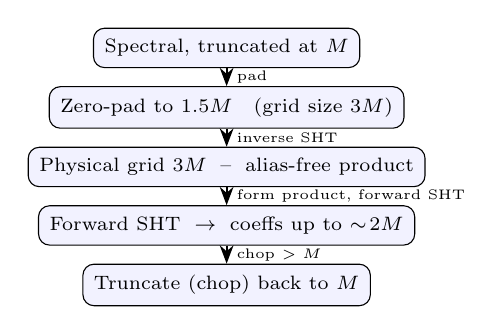
\begin{tikzpicture}[
        node distance=6.5pt,
        box/.style={draw, rounded corners, align=center, font=\scriptsize, inner sep=4pt, fill=blue!5},
        arr/.style={-{Stealth}, thick}]
        \node[box] (a) {Spectral, truncated at $M$};
        \node[box, below=of a] (b) {Zero-pad to $1.5M$ \; (grid size $3M$)};
        \node[box, below=of b] (c) {Physical grid $3M$ \;--\; alias-free product};
        \node[box, below=of c] (d) {Forward SHT \;$\to$\; coeffs up to $\sim\!2M$};
        \node[box, below=of d] (e) {Truncate (chop) back to $M$};
        \draw[arr] (a) -- node[right, font=\tiny] {pad} (b);
        \draw[arr] (b) -- node[right, font=\tiny] {inverse SHT} (c);
        \draw[arr] (c) -- node[right, font=\tiny] {form product, forward SHT} (d);
        \draw[arr] (d) -- node[right, font=\tiny] {chop $>M$} (e);
    \end{tikzpicture}
    \end{center}
    Implemented with a second, padded transform pair (\texttt{*\_d}) at $l_{\max}=\lceil 1.5M\rceil$,
    $n_{lat}=2l_{\max}$; toggled by the \texttt{dealias} flag. The clean, un-aliased coefficients
    (degree $\le M$) are returned to the integrator.
\end{frame}

\subsection{The Dilemma}
\begin{frame}{The Dilemma}
    \begin{itemize}
        \item The SFNO architecture is amazingly powerful in emulating on real-world data 
        \item Yet the same architecture fails to emulate a simple idealistic setup with:
        \begin{itemize}
            \item \textbf{Shallow Water Equation} as the primitive equation
            \item \textbf{Simple Initial Condition} : a barotropically instable zonal jet. 
        \end{itemize}
    \end{itemize}
\end{frame}

\begin{frame}{Potential Causes}
\begin{tcolorbox}[colframe=blue!60!white, title=Cause 1. Simulation is too short]

In the Fourcastnet training, we have reanalysis data for decades.Current dataset has duration of $\sim \text{15 days}$.

\end{tcolorbox}

\begin{tcolorbox}[colframe=blue!60!white, title=Cause 2. Samples lack the variability]

In the Fourcastnet training, all training samples are real world data. In training for Galewsky, all initial conditions is a simple, barotropically instable flow. 
\end{tcolorbox}
    
\end{frame}
\subsection{An Analogy}
\begin{frame}{An Analogy for Cause 2}
    In the case of interest, Neural operator is a mapping from the initial condition to the solution after $t$ seconds. In other word, they are a function:
    $$\mathcal A:TS^2 \times \mathbb{R}\to TS^2$$
    where $TS^2$ denotes the field on the sphere.

    Consider the simplest case of learning a map between $\mathbb{R}^3$. The ground truth map can be represented as a diagonal matrix:

    \begin{equation}
        A=\begin{pmatrix}
            \lambda _1 & &  \\
            & \lambda_2 & &\\
            & & \lambda_3  &
        \end{pmatrix}
    \end{equation}
    
\end{frame}

\begin{frame}{An Analogy for Cause 2(Continued)}
Suppose are training samples are located near the first eigenvector with eigenvalue $\lambda_1$: 
    \begin{figure}
        \centering
        \include{media/linear_analogy}
        \caption{$V$ is the domain, akin to initial conditions; $W$ is the codomain, akin to all possible solutions at time $t$; The bold balck vector is the eigenvector; Colorful vectors are the training samples}
        \label{fig:placeholder}
    \end{figure}
\end{frame}

\begin{frame}{An Analogy for Cause 2(Continued)}
Let $A^{\dagger}$ be the learned opeartor:
\begin{equation}
        A^{\dagger}=\begin{pmatrix}
            \mu _1 & &  \\
            & \mu_2 & &\\
            & & \mu_3  &
        \end{pmatrix}
\end{equation}
The learned operator would have $\mu_1 =\lambda_1 +\epsilon$ where $\epsilon$ can be made arbitrarily small. However $\mu_2, \mu_3$ would be basically noise.
\end{frame}

\begin{frame}{Why Cause 1 Might be Insignificant}
    The training for FourcastNet is, suprisingly, straightforward:
\begin{algorithm}[H]
\caption{Model Training Procedure}
\begin{algorithmic}[1]


\FOR{$\text{epoch} = 1$ \TO $80$}
    \FOR{each $\mathbf{X}(k) \in D_{\text{train}}$}
        \STATE $\hat{\mathbf{X}}(k+1) = \text{Model}(\mathbf{X}(k))$
        \STATE Backprop on $\mathcal{L} = \text{Loss}(\hat{\mathbf{X}}(k+1), \mathbf{X}_{\text{true}}(k+1))$
    \ENDFOR
\ENDFOR


\FOR{$\text{epoch} = 1$ \TO $50$}
    \FOR{each $\mathbf{X}(k) \in D_{\text{train}}$}
        \STATE $\hat{\mathbf{X}}(k+1) = \text{Model}(\mathbf{X}(k))$
        \quad  $\hat{\mathbf{X}}(k+2) = \text{Model}(\hat{\mathbf{X}}(k+1))$
    
        \STATE Backprop on $\mathcal L_1 +\mathcal L_2$
    \ENDFOR
\ENDFOR
\end{algorithmic}
\end{algorithm}

\end{frame}

\begin{frame}{Why Cause 1 Might be Insignificant(Continued)}
    \begin{itemize}
        \item From the psuedocode above, each sample is simply $(X^{(i)}(k),X^{(i)}(k+1))$ or $(X^{(i)}(k),X^{(i)}(k+1)),X^{(i)}(k+2))$. In other word, $X^{(i)}(k), X^{(i)}(k')$ where $k>k'+2$ is drawn independently from the distribution $D$.

        \item In addition, it is vastly challenging to ask for longer simulation since no numerical models can simulate Galewsky sufficiently long($\sim$ year) while still stay numerically convergent. The challenge is intrinsic to the complexity of bifurcation. 
    \end{itemize}
\end{frame}

\begin{frame}{Why Cause 1 Might be Hard to Resolve}

\begin{figure}[htbp]
    \centering
    \begin{minipage}[b]{0.48\textwidth}
        \centering
        \includegraphics[width=\textwidth]{media/numerical_convergence_1.png}
        \caption{$\tau=6,l_{max}=256$}

    \end{minipage}
    \hfill
    \begin{minipage}[b]{0.48\textwidth}
        \centering
        \includegraphics[width=\textwidth]{media/numerical_convergence_2.png}
        \caption{$\tau=6,l_{max}=256$}

    \end{minipage}
\end{figure}

\end{frame}

\subsection{"Real-World" Initial Condition}
\begin{frame}{"Real-World" Initial Condition}
    \begin{itemize}
        \item Idea: Try to construct more complex flows as initial conditions that has greater variability; 
        \item A Better Idea: Why not use real world data such as \textbf{ERA5 hourly data on pressure levels}
    \end{itemize}


\begin{algorithm}[H]
\caption{RWIC Generation}
    \begin{algorithmic}[1]
        \STATE Randomly pick $t\in T$, extract $(u_t,v_t)$
        \STATE Compute $(\hat \zeta_t,\hat \delta_t)$
        \STATE Compute $\Phi_t$ via the non-linear balance equation:
        $$\nabla^2 \Phi = \nabla \times \left[ \mathbf{u}(\zeta + f) \right] - \nabla^2 K$$
        where $K$ is kinetic energy
        \RETURN $(\hat \Phi_t, \hat \zeta, \hat \delta)$
    \end{algorithmic}
\end{algorithm}

\end{frame}

\begin{frame}{RWIC Example}
    \begin{figure}
        \centering
        \includegraphics[width=1.02\linewidth]{media/initial_condition_sphere.png}
        \caption{Example RWIC}
        \label{fig:placeholder}
    \end{figure}
\end{frame}


\begin{frame}{RWIC Example Run}

\end{frame}

\end{document}